%===============================================================================
% LaTeX sjabloon voor de bachelorproef toegepaste informatica aan HOGENT
% Meer info op https://github.com/HoGentTIN/latex-hogent-report
%===============================================================================

\documentclass[dutch,dit,thesis]{hogentreport}

% TODO:
% - If necessary, replace the option `dit`' with your own department!
%   Valid entries are dbo, dbt, dgz, dit, dlo, dog, dsa, soa
% - If you write your thesis in English (remark: only possible after getting
%   explicit approval!), remove the option "dutch," or replace with "english".

\usepackage{lipsum} % For blind text, can be removed after adding actual content

%% Pictures to include in the text can be put in the graphics/ folder
\graphicspath{{../graphics/}}

%% For source code highlighting, requires pygments to be installed
%% Compile with the -shell-escape flag!
%% \usepackage[chapter]{minted}
%% If you compile with the make_thesis.{bat,sh} script, use the following
%% import instead:
\usepackage[chapter,outputdir=../output]{minted}
\usemintedstyle{solarized-light}

%% Formatting for minted environments.
\setminted{%
    autogobble,
    frame=lines,
    breaklines,
    linenos,
    tabsize=4
}

%% Ensure the list of listings is in the table of contents
\renewcommand\listoflistingscaption{%
    \IfLanguageName{dutch}{Lijst van codefragmenten}{List of listings}
}
\renewcommand\listingscaption{%
    \IfLanguageName{dutch}{Codefragment}{Listing}
}
\renewcommand*\listoflistings{%
    \cleardoublepage\phantomsection\addcontentsline{toc}{chapter}{\listoflistingscaption}%
    \listof{listing}{\listoflistingscaption}%
}

% Other packages not already included can be imported here

%%---------- Document metadata -------------------------------------------------
% TODO: Replace this with your own information
\author{Stefan De Moor}
\supervisor{Mevr. F. Spriet}
\cosupervisor{Dhr. G. Bettens}
\title{Onderzoek en concept ontwikkeling\\mobile app voor een Energy\\Management System.}
\academicyear{\advance\year by -1 \the\year--\advance\year by 1 \the\year}
\examperiod{1}
\degreesought{\IfLanguageName{dutch}{Professionele bachelor in de toegepaste informatica}{Bachelor of applied computer science}}
\partialthesis{false} %% To display 'in partial fulfilment'
%\institution{Internshipcompany BVBA.}

%% Add global exceptions to the hyphenation here
\hyphenation{back-slash}

%% The bibliography (style and settings are  found in hogentthesis.cls)
\addbibresource{bachproef.bib}            %% Bibliography file
\addbibresource{../voorstel/voorstel.bib} %% Bibliography research proposal
\defbibheading{bibempty}{}

%% Prevent empty pages for right-handed chapter starts in twoside mode
\renewcommand{\cleardoublepage}{\clearpage}

\renewcommand{\arraystretch}{1.2}

%% Content starts here.
\begin{document}

%---------- Front matter -------------------------------------------------------

\frontmatter

\hypersetup{pageanchor=false} %% Disable page numbering references
%% Render a Dutch outer title page if the main language is English
\IfLanguageName{english}{%
    %% If necessary, information can be changed here
    \degreesought{Professionele Bachelor toegepaste informatica}%
    \begin{otherlanguage}{dutch}%
       \maketitle%
    \end{otherlanguage}%
}{}

%% Generates title page content
\maketitle
\hypersetup{pageanchor=true}

%%=============================================================================
%% Voorwoord
%%=============================================================================

\chapter*{\IfLanguageName{dutch}{Woord vooraf}{Preface}}%
\label{ch:voorwoord}

%% TODO:
%% Het voorwoord is het enige deel van de bachelorproef waar je vanuit je
%% eigen standpunt (``ik-vorm'') mag schrijven. Je kan hier bv. motiveren
%% waarom jij het onderwerp wil bespreken.
%% Vergeet ook niet te bedanken wie je geholpen/gesteund/... heeft

\lipsum[1-2]
%%=============================================================================
%% Samenvatting
%%=============================================================================

% TODO: De "abstract" of samenvatting is een kernachtige (~ 1 blz. voor een
% thesis) synthese van het document.
%
% Een goede abstract biedt een kernachtig antwoord op volgende vragen:
%
% 1. Waarover gaat de bachelorproef?
% 2. Waarom heb je er over geschreven?
% 3. Hoe heb je het onderzoek uitgevoerd?
% 4. Wat waren de resultaten? Wat blijkt uit je onderzoek?
% 5. Wat betekenen je resultaten? Wat is de relevantie voor het werkveld?
%
% Daarom bestaat een abstract uit volgende componenten:
%
% - inleiding + kaderen thema
% - probleemstelling
% - (centrale) onderzoeksvraag
% - onderzoeksdoelstelling
% - methodologie
% - resultaten (beperk tot de belangrijkste, relevant voor de onderzoeksvraag)
% - conclusies, aanbevelingen, beperkingen
%
% LET OP! Een samenvatting is GEEN voorwoord!

%%---------- Nederlandse samenvatting -----------------------------------------
%
% TODO: Als je je bachelorproef in het Engels schrijft, moet je eerst een
% Nederlandse samenvatting invoegen. Haal daarvoor onderstaande code uit
% commentaar.
% Wie zijn bachelorproef in het Nederlands schrijft, kan dit negeren, de inhoud
% wordt niet in het document ingevoegd.

\IfLanguageName{english}{%
\selectlanguage{dutch}
\chapter*{Samenvatting}
\lipsum[1-4]
\selectlanguage{english}
}{}

%%---------- Samenvatting -----------------------------------------------------
% De samenvatting in de hoofdtaal van het document

\chapter*{\IfLanguageName{dutch}{Samenvatting}{Abstract}}

Dit onderzoek richt zich op de ontwikkeling van een mobiele applicatie voor het energiebeheersysteem SmartKit van ATS, dat energiestromen zoals zonnepanelen, batterijen, laadpalen en verwarming monitort en aanstuurt. Het doel is de huidige communicatie van systeemmeldingen en foutmeldingen, die nu via e-mail plaatsvinden, te verbeteren door deze om te zetten naar mobiele notificaties, zodat gebruikers sneller en efficiënter geïnformeerd worden. Het onderzoek onderzoekt welke technologie het meest geschikt is voor de ontwikkeling van een kostenefficiënte en schaalbare app. Drie benaderingen worden vergeleken: native apps, Progressive Web Apps (PWA), en cross-platform frameworks (zoals React Native en Flutter). \\

De centrale onderzoeksvraag is: "Welke benadering is het meest geschikt voor de ontwikkeling van de mobiele app en hoe kan deze op een veilige manier user management en notificaties integreren?" De methodologie omvat een literatuurstudie over de verschillende technologieën, gevolgd door de ontwikkeling van een Proof of Concept (POC) om de haalbaarheid van de gekozen oplossing te testen. De verwachte resultaten zijn een gedetailleerde vergelijking van de technische mogelijkheden van de benaderingen, evenals een werkend prototype van de app. \\

Voor de Proof of Concept werd gekozen om de app te ontwikkelen met het cross-platform framework .NET MAUI, vanwege de goede ondersteuning voor zowel Android als iOS, de integratie met C# (waar het bedrijf al ervaring mee heeft), en de flexibiliteit op vlak van back-end koppeling. In het testproject werden essentiële functies uitgewerkt zoals gebruikersauthenticatie met JWT, veilige opslag via Secure Storage, en pushnotificaties via Firebase. Uit de tests blijkt dat deze technieken niet alleen technisch haalbaar zijn, maar ook vlot werken binnen een mobiele context. Hoewel de POC niet werd geïntegreerd in SmartKit zelf, tonen de resultaten aan dat de gekozen benadering veelbelovend is. De implementatie op kleine schaal laat toe om in een volgende fase met meer zekerheid en minder risico de overstap naar het echte product te maken. Verdere stappen richting integratie in SmartKit vereisen wel bijkomend werk zoals diepgaandere tests, afstemming met bestaande systemen en gebruikersfeedback.


%---------- Inhoud, lijst figuren, ... -----------------------------------------

\tableofcontents

% In a list of figures, the complete caption will be included. To prevent this,
% ALWAYS add a short description in the caption!
%
%  \caption[short description]{elaborate description}
%
% If you do, only the short description will be used in the list of figures

\listoffigures

% If you included tables and/or source code listings, uncomment the appropriate
% lines.
\listoftables

\listoflistings

% Als je een lijst van afkortingen of termen wil toevoegen, dan hoort die
% hier thuis. Gebruik bijvoorbeeld de ``glossaries'' package.
% https://www.overleaf.com/learn/latex/Glossaries

%---------- Kern ---------------------------------------------------------------

\mainmatter{}

% De eerste hoofdstukken van een bachelorproef zijn meestal een inleiding op
% het onderwerp, literatuurstudie en verantwoording methodologie.
% Aarzel niet om een meer beschrijvende titel aan deze hoofdstukken te geven of
% om bijvoorbeeld de inleiding en/of stand van zaken over meerdere hoofdstukken
% te verspreiden!

%%=============================================================================
%% Inleiding
%%=============================================================================

\chapter{\IfLanguageName{dutch}{Inleiding}{Introduction}}%
\label{ch:inleiding}

\noindent In een wereld waarin energiebeheer steeds belangrijker wordt, speelt efficiënte monitoring en besturing van energiestromen een cruciale rol. Het SmartKit-systeem van ATS is ontworpen om deze energiestromen, waaronder zonnepanelen, batterijen, laadpalen en verwarmingssystemen, te beheren. Momenteel worden systeemmeldingen, zoals storingen of operationele statusupdates, via e-mail gecommuniceerd. Dit leidt echter tot een overdaad aan berichten, waardoor kritieke meldingen over het hoofd kunnen worden gezien. Een effectievere oplossing is nodig om real-time meldingen beter te beheren en de respons op systeemstoringen te versnellen. \\

\section{\IfLanguageName{dutch}{Probleemstelling}{Problem Statement}}%
\label{sec:probleemstelling}

\noindent Dit onderzoek richt zich op de ontwikkeling van een mobiele applicatie voor SmartKit die meldingen efficiënter en veiliger naar de juiste gebruikers stuurt via mobiele notificaties. Een dergelijke applicatie kan de beheerders van het systeem in staat stellen sneller en gerichter te reageren, wat de algehele efficiëntie en betrouwbaarheid van het systeem verbetert. \\

\section{\IfLanguageName{dutch}{Onderzoeksvraag}{Research question}}%
\label{sec:onderzoeksvraag}

\noindent De centrale onderzoeksvraag luidt:

\begin{quote} 
    \textit{Welke technologie is het meest geschikt voor de ontwikkeling van een mobiele applicatie die systeemmeldingen efficiënt en veilig verstuurt, en hoe kan deze technologie op een kostenefficiënte manier worden geïntegreerd met het bestaande SmartKit-systeem?} 
\end{quote}

\noindent Om deze vraag te beantwoorden, worden verschillende aspecten van mobiele applicatieontwikkeling onderzocht. Dit leidt tot de volgende deelvragen:

\begin{itemize}
    \item Wat zijn de voor- en nadelen van native apps, Progressive Web Apps (PWA) en cross-platform frameworks voor de ontwikkeling van de mobiele applicatie? Hierbij wordt gekeken naar prestaties, gebruikservaring en ontwikkeltijd.
    
    \item Hoe kan de mobiele applicatie op een veilige manier gebruikers beheren en toegang reguleren? Dit omvat aspecten zoals authenticatie en autorisatie, die essentieel zijn om gevoelige systeemdata binnen het SmartKit-systeem te beschermen.
    
    \item Welke technologieën zijn het meest geschikt voor het efficiënt versturen van mobiele notificaties binnen de gekozen ontwikkelstrategie? Hierbij wordt onderzocht welke pushnotificatietechnologieën geschikt zijn voor real-time communicatie en hoe deze kunnen worden geïntegreerd binnen het SmartKit-systeem.
    
    \item Wat zijn de kosten- en schaalvoordelen van de meest geschikte technologie in de context van een klein ontwikkelteam? Dit aspect richt zich op de praktische haalbaarheid, implementatiekosten en onderhoud van de applicatie.
\end{itemize}

\noindent Op basis van dit onderzoek zal één technologie geselecteerd worden voor verdere uitwerking. Daarbij wordt onder andere .NET MAUI als mogelijke optie verder onderzocht en geëvalueerd.


\section{\IfLanguageName{dutch}{Onderzoeksdoelstelling}{Research objective}}%
\label{sec:onderzoeksdoelstelling}

\noindent De doelstelling van dit onderzoek is om een technologisch onderbouwde keuze te maken voor de ontwikkeling van een mobiele applicatie die de communicatie van SmartKit-meldingen optimaliseert. Dit zal resulteren in een gedetailleerd onderzoeksrapport en een Proof of Concept (PoC) die de geselecteerde technologieën in de praktijk demonstreert. De uitkomsten van dit onderzoek zullen bijdragen aan een verbeterde werking van het SmartKit-systeem, een efficiëntere afhandeling van systeemmeldingen en een verhoogde klanttevredenheid. \\

\section{\IfLanguageName{dutch}{Opzet van deze bachelorproef}{Structure of this bachelor thesis}}%
\label{sec:opzet-bachelorproef}

TODO


\chapter{\IfLanguageName{dutch}{Stand van zaken}{State of the art}}
\label{ch:stand-van-zaken}

\section{Inleiding}
In dit hoofdstuk wordt een overzicht gegeven van de huidige stand van zaken rondom mobiele applicatieontwikkeling. De focus ligt daarbij op beveiliging, de keuze van platformen en cross-platform technologieën. Het doel is om de technologische context van dit project helder in kaart te brengen, zodat er een weloverwogen keuze kan worden gemaakt voor het meest geschikte ontwikkelplatform. Door recente ontwikkelingen en relevante literatuur te bespreken, leggen we een stevige basis voor de onderzoeksvragen en ontwerpbeslissingen die hierop volgen.

\section{Vergelijking van mobiele ontwikkelstrategieën}

Mobiele applicaties kunnen op uiteenlopende manieren worden ontwikkeld, afhankelijk van factoren zoals doelstellingen, budget, gewenste gebruikerservaring en technische vereisten. De keuze voor een specifieke ontwikkelstrategie is vaak bepalend voor het succes van een mobiele toepassing. Elke aanpak brengt namelijk eigen afwegingen met zich mee op het gebied van prestaties, onderhoud, ontwikkelsnelheid en compatibiliteit met verschillende platformen \autocite{Sharma2025}.\\

In deze sectie worden drie gangbare benaderingen uiteengezet: \textit{native development}, \textit{progressive web apps} (PWA’s) en \textit{cross-platform development}. Het doel is om een helder inzicht te geven in de principes van deze strategieën, zonder daarbij al in te gaan op specifieke tools of frameworks die komen later aan bod.\\

De bespreking en vergelijking van deze strategieën vindt plaats aan de hand van meerdere relevante criteria, waaronder prestaties, gebruikservaring, onderhoudsgemak, ontwikkelkosten en time-to-market. Deze analyse vormt de inhoudelijke basis voor het bepalen van de meest geschikte ontwikkelrichting binnen dit project.



\subsection{Native apps}
Een native app is een mobiele applicatie die specifiek is ontworpen voor een bepaald besturingssysteem of platform, zoals Android of iOS. Deze apps worden gebouwd met behulp van programmeertalen en ontwikkeltools die specifiek zijn voor dat platform. Voor Android zijn dat bijvoorbeeld Kotlin of Java, en voor iOS Swift of Objective-C. Native apps worden geïnstalleerd via de officiële appstores (Google Play of App Store) en draaien rechtstreeks op het besturingssysteem van het apparaat \autocite{Singh2024}.\\

Het grote voordeel van deze aanpak is dat native apps volledig kunnen profiteren van de functies van het besturingssysteem en de hardware van het apparaat. Denk hierbij aan toegang tot de camera, GPS, pushmeldingen, en een native gebruikersinterface. Volgens \textcite{Gillis2022} levert deze vorm van appontwikkeling de beste prestaties en de diepste integratie met het platform.\\

Een belangrijk voordeel is dat native apps een optimale gebruikerservaring bieden: ze voelen als een natuurlijk onderdeel van het platform, laden snel, tonen vloeiende animaties en volgen consistente interactiepatronen \autocite{Gillis2022}. Daartegenover staat dat deze aanpak vaak aparte ontwikkelteams per platform vereist, wat kan leiden tot hogere kosten en een langere time-to-market.

\subsection{Progressive Web Apps (PWA)}  
Progressive Web Apps zijn webapplicaties die zich gedragen als native apps. Ze maken gebruik van moderne webtechnologieën zoals HTML5, CSS3 en JavaScript, in combinatie met service workers en manifest-bestanden. PWA’s draaien in een browseromgeving, maar kunnen ook offline functioneren, pushnotificaties versturen en op het startscherm van een toestel worden geplaatst. PWA’s laden bij de eerste keer de volledige applicatie in en functioneren daarna vrijwel zelfstandig, zelfs bij slechte of afwezige internetverbindingen \autocite{Hendriksen2020}.\\

De belangrijkste voordelen van PWA’s zijn hun platformonafhankelijkheid en relatief lage ontwikkelkosten: één codebase is voldoende voor alle apparaten met een moderne browser. De functionaliteit is echter beperkter dan bij native apps, vooral wat betreft toegang tot hardware en beveiligde API’s.\\  

Een API (Application Programming Interface) is een software-interface die ervoor zorgt dat verschillende applicaties met elkaar kunnen communiceren. Je kunt het vergelijken met een ober in een restaurant: jij geeft een bestelling door, de ober neemt die bestelling mee naar de keuken (de server) en brengt het bereide gerecht terug naar jou. Op deze manier kunnen applicaties via API’s data opvragen en uitwisselen zonder dat zij direct toegang hebben tot elkaars systemen \autocite{Schoemaker2019}.\\  

Bij PWA’s worden API’s bijvoorbeeld gebruikt om informatie op te halen, zoals gebruikersdata, pushnotificaties te versturen of betalingen te verwerken. Omdat iOS nog beperkingen kent op bepaalde API-functionaliteiten, werkt niet alle functionaliteit in een PWA op iPhones even volledig als op Android.\\  

De markt voor PWA’s groeit snel. In 2023 werd de wereldwijde marktwaarde geschat op 1,46 miljard USD, met een verwachte jaarlijkse groei van 31,1 procent tussen 2024 en 2030 \autocite{Research2024}. Deze groei wordt gedreven door factoren zoals de toenemende internetpenetratie en de vraag naar snelle, toegankelijke mobiele ervaringen. Grote bedrijven zoals Tinder, X (voorheen Twitter) en Forbes maken al gebruik van PWA-technologie. Figuur~\ref{fig:pwa_market} toont de verwachte marktgroei tot 2030.\\  


\begin{figure}[h]
    \centering
    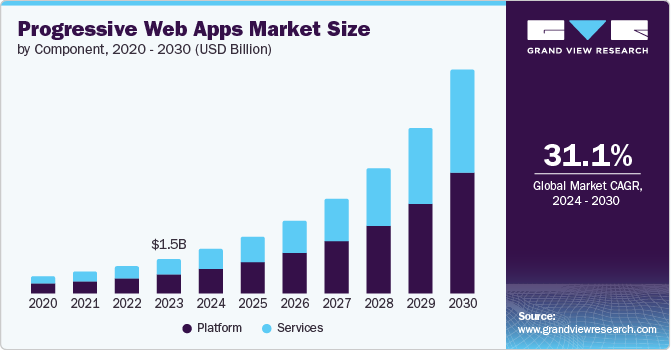
\includegraphics[width=0.75\textwidth]{pwa-market.png}
    \caption{Wereldwijde marktgroei van Progressive Web Apps (USD miljard), 2020–2030. Bron: Grand View Research, 2025. \autocite{Research2024}}
    \label{fig:pwa_market}
\end{figure}

\subsection{Cross-platform frameworks}
Cross-platform frameworks zoals Flutter, React Native en .NET MAUI vormen een middenweg tussen de prestaties van native apps en de snelle ontwikkeltijd van PWA’s. Ze maken het mogelijk om met één gedeelde codebase applicaties te ontwikkelen voor meerdere platformen, wat de ontwikkeltijd verkort en onderhoudskosten verlaagt \autocite{Kuppan2024}.\\

Flutter en React Native gebruiken eigen rendering-engines of native componenten voor de gebruikersinterface, terwijl .NET MAUI direct platform-native UI-elementen aanspreekt via .NET-technologie. Uit onderzoek blijkt dat Flutter uitblinkt in vloeiende animaties en UI-prestaties, terwijl .NET MAUI sterk is in integratie met Microsoft-omgevingen \autocite{Gajjam2025}. Toch blijven cross-platform apps soms iets achter bij native apps, vooral bij grafisch intensieve of rekenintensieve toepassingen.

\begin{table}[h]
    \centering
    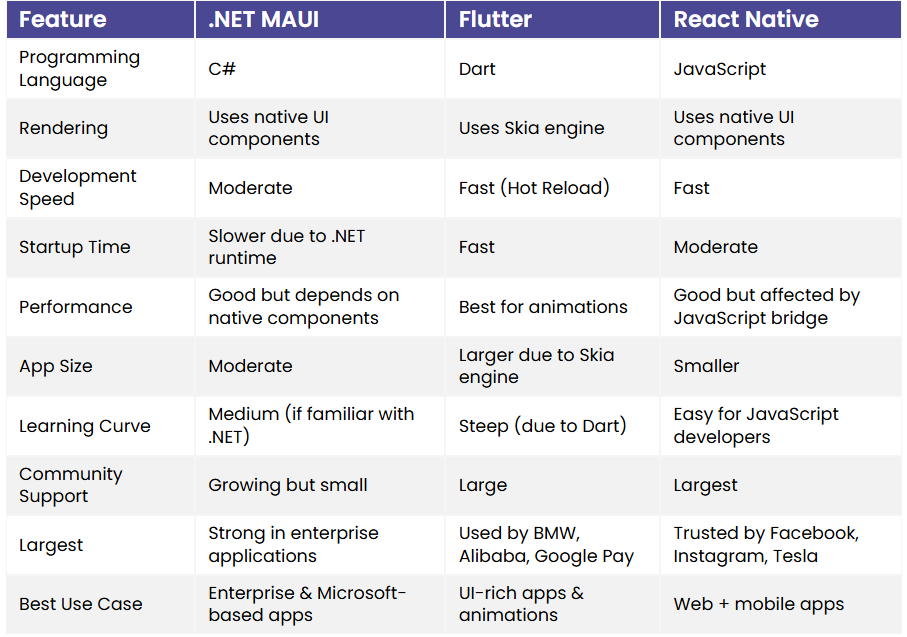
\includegraphics[width=0.8\textwidth]{comparison1.png}
    \caption[Integratie]{Vergelijking van .NET MAUI, Flutter en React Native op basis van geschiktheid voor enterprise-omgevingen \autocite{Gajjam2025}}
    \label{fig:vergelijking}
\end{table}

\begin{table}[h]
    \centering
    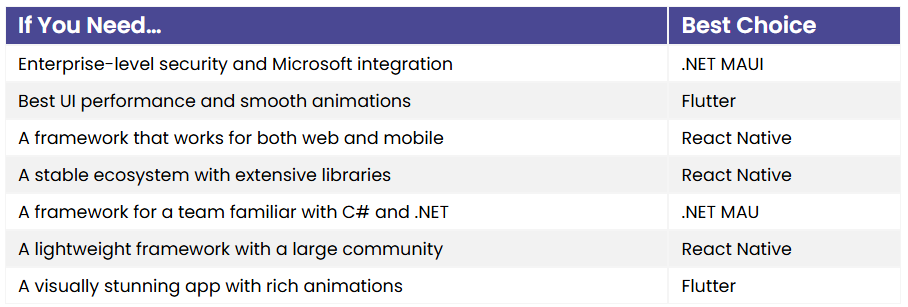
\includegraphics[width=0.8\textwidth]{comparison2.png}
    \caption[Frameworkkeuze]{Overzicht van aanbevolen cross-platform frameworks (Flutter, React Native en .NET MAUI) op basis van specifieke projectvereisten \autocite{Gajjam2025}}
    \label{tab:frameworkkeuze}
\end{table}

\subsection{Samenvatting en aanbevelingen}
Welke mobiele ontwikkelstrategie het beste past, hangt af van de context, de doelstellingen en de technische randvoorwaarden van het project. Uit voorgaand onderzoek blijkt dat native apps bijzonder geschikt zijn voor toepassingen waarbij maximale prestaties en een hoogwaardige gebruikerservaring cruciaal zijn, bijvoorbeeld bij games of apps met intensieve interactie \autocite{Singh2024, Gillis2022}. Deze aanpak zorgt voor optimale integratie met het besturingssysteem en directe hardwaretoegang, maar vergt vaak aparte teams per platform, wat hogere kosten en een langere ontwikkeltijd tot gevolg heeft.\\

Progressive Web Apps bieden een kosteneffectieve, platformonafhankelijke oplossing, met één codebase voor alle moderne browsers. Ze zijn geschikt voor eenvoudige of informatieve apps zonder complexe functies. De functionaliteit is echter beperkter, vooral wat betreft hardwaretoegang en beveiligde API’s. Ook is de ondersteuning voor bepaalde functies, zoals pushnotificaties op iOS, nog beperkt.\\

Cross-platform frameworks als Flutter, React Native en .NET MAUI vormen een aantrekkelijk compromis: met één gedeelde codebase kunnen apps voor meerdere platformen worden ontwikkeld, wat de ontwikkeltijd verkort en het onderhoud vereenvoudigt. Flutter onderscheidt zich door uitstekende UI-prestaties en animaties, terwijl .NET MAUI een goede keuze is voor organisaties die diep in het Microsoft-ecosysteem zitten, mede dankzij de integratie met Visual Studio en Azure.\\

Figuur~\ref{fig:vergelijking} toont een overzicht van de voor- en nadelen van deze strategieën. De beste keuze hangt af van het doel van de app, de gewenste gebruikerservaring en de beschikbare middelen. Zo is .NET MAUI vaak de beste optie in enterprise-omgevingen waar stabiliteit, veiligheid en integratie centraal staan, terwijl native ontwikkeling of PWA’s beter kunnen passen bij specifieke projectdoelen en budgetten.\\

Kortom, door zorgvuldig af te wegen tussen prestaties, ontwikkeltijd, functionaliteit en de organisatorische context, kan een projectteam een mobiele ontwikkelstrategie kiezen die zowel aan technische als zakelijke eisen voldoet.

\section{Vergelijking van Cross-Platform Frameworks}

\subsection{Wat is een UI-framework?}
Een UI-framework (User Interface framework) is een verzameling vooraf gebouwde, herbruikbare componenten, stijlen en tools die het ontwikkelen van gebruikersinterfaces vereenvoudigt en versnelt. Denk hierbij aan standaardcomponenten zoals knoppen, formulieren en navigatiebalken, die consequent zijn vormgegeven en functioneren. UI-frameworks zorgen voor ontwerpconsistentie binnen een applicatie, versnellen het ontwikkelproces en zijn vaak responsief ontworpen, zodat applicaties goed werken op verschillende apparaten en schermformaten \autocite{Coditation2023}.\\

Het gebruik van een UI-framework brengt voordelen met zich mee, zoals snellere ontwikkeling, een uniforme gebruikerservaring en toegang tot een actieve community voor ondersteuning. Tegelijkertijd kunnen sommige frameworks ook beperkingen opleveren, bijvoorbeeld qua performance of aanpasbaarheid, afhankelijk van de projectbehoeften.\\

\subsection{Flutter}
Flutter is een open-source UI-framework van Google, gebaseerd op de programmeertaal Dart. Het staat bekend om hoge prestaties, vloeiende animaties en een uitgebreide set widgets, die dienen als de visuele en interactieve onderdelen van een app. Een widget kan bijvoorbeeld een knop, een tekstveld of een menu zijn, en vormt steeds een klein stukje van de gebruikersinterface. Door deze widgets slim te combineren, kunnen ontwikkelaars op een eenvoudige manier professionele en consistente apps bouwen. Daarnaast biedt Flutter ondersteuning voor plug-ins, die extra mogelijkheden toevoegen aan een app zonder dat deze volledig zelf ontwikkeld hoeven te worden. Denk hierbij aan functies zoals het openen van de camera, het bepalen van de locatie of het opslaan van gegevens op het toestel. Flutter ondersteunt iOS, Android, web en desktop, en profiteert van een groeiende community met een grote hoeveelheid beschikbare widgets en plug-ins \autocite{Gajjam2025}.\\

Een onderscheidend kenmerk is \emph{hot reload}, dit betekent dat ontwikkelaars realtime wijzigingen kunnen doorvoeren. Wat de ontwikkelsnelheid sterk verhoogt. Flutter ondersteunt zowel Material Design als Cupertino-stijl en maakt gebruik van de Skia-renderengine voor consistente prestaties \autocite{Rodriguez2025}.\\

In 2023 gebruikte 46\% van ontwikkelaars wereldwijd Flutter, waarmee het het populairste cross-platform framework is. Grote merken zoals Google Ads, BMW en Alibaba vertrouwen op Flutter, wat de kracht van één codebase en besparingen in tijd en kosten benadrukt. Figuur~\ref{fig:flutter} toont een overzicht van het gebruik van verschillende frameworks.\\

Een beperking is de matige integratie met enterprise-systemen en Microsoft-\\technologieën, wat voor organisaties die sterk op het Microsoft-ecosysteem\\ steunen een nadeel kan zijn.

\subsection{React Native}
React Native, ontwikkeld door Meta, maakt het mogelijk mobiele apps te bouwen met JavaScript en React. Het biedt een goede balans tussen snelheid, performance en schaalbaarheid, zeker in combinatie met het Expo-platform dat native build-omgevingen vereenvoudigt \autocite{Ivanov2025}.\\

Met één codebase voor iOS en Android worden ontwikkeltijden verkort en kosten gedrukt, wat vooral aantrekkelijk is voor kleine teams. Expo voegt hier hot reloading en een managed workflow aan toe, plus de Expo Go-app voor directe testing op fysieke apparaten \autocite{Ivanov2025}.\\

Een managed workflow betekent dat veel technische details automatisch voor je worden geregeld. Hierdoor kunnen ontwikkelaars zich vooral richten op het schrijven van de app zelf, zonder zich zorgen te maken over ingewikkelde instellingen of installatieproblemen. Dit maakt het ontwikkelen makkelijker en sneller, vooral voor teams die niet veel tijd of ervaring hebben met het bouwen van apps.\\

React Native maakt het mogelijk om apps te bouwen die aanvoelen alsof ze speciaal voor een bepaald toestel zijn gemaakt. Dit gebeurt doordat de technologie contact maakt met functies van het toestel zelf, zoals de camera of het touchscreen. Bewegingen en overgangen in de app, zoals het schuiven van een menu of het openen van een scherm, verlopen meestal soepel dankzij speciale hulpmiddelen voor animaties \autocite{Ivanov2025}. Dankzij zogenaamde Over-the-Air updates, waarbij de aanpassingen draadloos via het internet naar de app worden gestuurd, kunnen kleine veranderingen of foutoplossingen snel bij gebruikers terechtkomen zonder dat de app opnieuw via de appwinkel hoeft te worden gedownload.\\

Echter, voor complexe platform-specifieke functies is vaak native code nodig, wat extra onderhoud vergt. De integratie met Microsoft-technologieën is beperkt, waardoor .NET MAUI vaak de voorkeur heeft in enterprise-omgevingen met Azure en .NET-backends \autocite{Longe2025}.

\subsection{.NET MAUI}
.NET MAUI, de opvolger van Xamarin, is Microsofts nieuwste cross-platform framework. Het stelt ontwikkelaars in staat met één codebase apps te bouwen voor iOS, Android, Windows en macOS, wat kosten en onderhoud reduceert \autocite{Sheth2024}.\\

De diepe integratie met het Microsoft-ecosysteem (Visual Studio, Azure, .NET Core) zorgt voor uniforme tooling, samenwerking en toegang tot uitgebreide documentatie \autocite{Sheth2024}. Visual Studio ondersteunt functies als Hot Reload en Live Preview voor een snelle ontwikkelcyclus.\\

Dankzij een enkele projectstructuur maakt .NET MAUI het makkelijker om apps voor verschillende apparaten te ontwikkelen. De gebruiksvensters en knoppen passen zich automatisch aan het besturingssysteem aan \autocite{Sheth2024}. Hierdoor krijgt de gebruiker overal een gelijkwaardige ervaring, terwijl het uiterlijk van het merk behouden blijft.\\

Performance is sterk dankzij efficiënt geheugenbeheer, snelle opstarttijden en directe toegang tot native API’s. Platform-specifieke extensies zijn mogelijk via custom handlers zonder de gedeelde codebasis te verlaten.\\

Voor organisaties die zwaar investeren in Microsoft-technologieën biedt .NET MAUI een strategisch voordeel door naadloze integratie met ASP.NET Core en Azure App Services \autocite{Klesman2023}.

\begin{figure}[h]
    \centering
    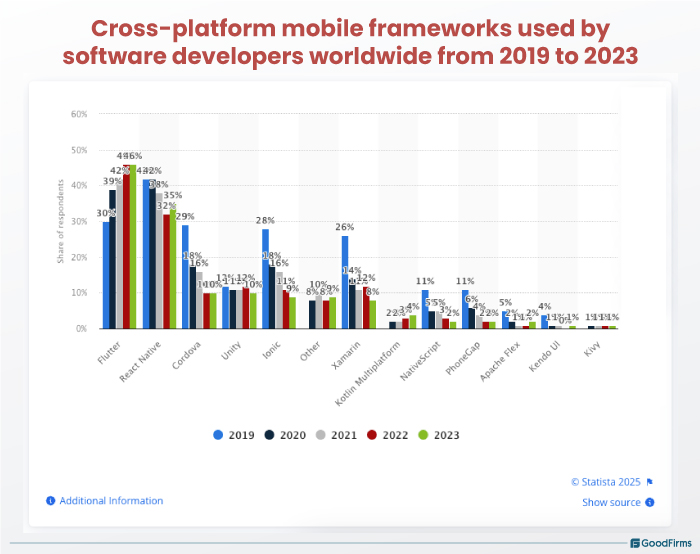
\includegraphics[width=0.75\textwidth]{flutter.jpg}
    \caption{Gebruik van cross-platform frameworks onder ontwikkelaars in 2023. Bron: Statista \autocite{Rodriguez2025}}
    \label{fig:flutter}
\end{figure}

\subsection{Technologische Continuïteit}
Gezien ATS reeds intensief werkt met het .NET-ecosysteem (C#, ASP.NET Core, Azure), sluit .NET MAUI optimaal aan. Dit vermindert de leercurve, vereenvoudigt integratie en onderhoud, terwijl Flutter en React Native aanvullende kennis en inspanning vereisen \autocite{Longe2025}.

\subsection{Samenvatting en Aanbeveling}
Flutter, React Native en .NET MAUI bieden elk unieke voordelen. Flutter is ideaal voor visueel rijke apps en snelle ontwikkeling, React Native voor brede platformondersteuning en een grote community, terwijl .NET MAUI uitblinkt in integratie met Microsoft-technologie en enterprise-functionaliteit.\\

Voor een organisatie met sterke Microsoft-voorkeur en enterprise-eisen is .NET MAUI de beste keuze, dankzij technologische continuïteit, hergebruik van kennis en consistente gebruikerservaring.

\section{Moderne Authenticatie en Beveiligingspraktijken}

\subsection{Vergelijking van moderne authenticatiemethoden}

Mobiele authenticatie is belangrijk om te zorgen dat alleen geautoriseerde gebruikers toegang krijgen tot gevoelige gegevens en diensten op hun mobiele apparaten. Er bestaan verschillende methoden, elk met eigen voor- en nadelen.\\

Een veelgebruikte methode is sessiegebaseerde authenticatie. Hierbij houdt de server bij wie er is ingelogd door een tijdelijke sessie aan te maken. Dit werkt goed, maar kan problemen geven wanneer er veel gebruikers zijn, omdat de server al die sessies moet beheren \autocite{Gao2023}.\\

OAuth2 is een systeem dat vaak gebruikt wordt om gebruikers via één account toegang te geven tot meerdere diensten (bijvoorbeeld inloggen met je Google-account op andere websites). Dit heet ook wel federatieve toegang. OAuth2 is krachtig maar relatief ingewikkeld, en daarom soms minder geschikt voor eenvoudige apps die alleen intern gebruikt worden \autocite{Gao2023}.\\

JSON Web Tokens (JWT) zijn een lichtere en flexibelere manier om authenticatie te regelen. Hierbij worden gegevens over de gebruiker opgeslagen in een digitaal token dat de gebruiker meebrengt bij elk verzoek. Omdat de server deze tokens niet hoeft bij te houden, werkt het sneller en is het makkelijker schaalbaar. Dit maakt JWT populair in moderne systemen zoals cloudomgevingen en microservices \autocite{Gao2023}.\\

Naast deze methoden voor het vaststellen wie toegang krijgt, zijn er verschillende manieren om de identiteit van de gebruiker te controleren. De meest traditionele methode is het gebruik van wachtwoorden, waarbij gebruikers een geheime code invoeren. Hoewel dit veel voorkomt, zijn wachtwoorden kwetsbaar voor aanvallen zoals raden of diefstal \autocite{Zukarnain2022}.\\

Een veiliger alternatief is dynamische wachtwoorden, bijvoorbeeld via een sms-code. Hierbij krijgt de gebruiker een eenmalige code op zijn telefoon, die hij moet invoeren. Dit vermindert het risico op misbruik, maar sms-berichten kunnen onderschept worden \autocite{Zukarnain2022}.\\

Biometrische authenticatie maakt gebruik van unieke lichaamskenmerken zoals een vingerafdruk of gezichtsherkenning. Dit is handig omdat het snel en gebruiksvriendelijk is, en deze kenmerken moeilijk te vervalsen zijn. Toch is het een risico als biometrische data gelekt worden, want die kunnen niet veranderd worden zoals een wachtwoord \autocite{Zukarnain2022}.\\

Er zijn ook vernieuwende methoden zoals trajectgebaseerde authenticatie, waarbij het systeem kijkt naar de gebruikelijke reisroutes van een persoon om te controleren of het echt de juiste gebruiker is. Dit werkt minder goed voor mensen die vaak reizen of van locatie wisselen \autocite{Zukarnain2022}.\\

Verder is het belangrijk dat verschillende partijen, zoals mobiele netwerkproviders (operators), tussenpersonen (aggregators) en app-aanbieders (merchants), samenwerken. Zij hebben elk hun eigen beveiligingsmethodes, wat de situatie complex maakt. Het samenbrengen van al deze methoden op één platform kan de veiligheid verhogen en het beheer vereenvoudigen \textcite{Zukarnain2022}.\\

Kortom, mobiele authenticatie is een ingewikkeld vakgebied waarbij veiligheid, gebruiksgemak en snelheid goed in balans moeten worden gehouden \autocite{Zukarnain2022, Gao2023}.\\


\subsection{Overwegingen bij wachtwoordbeveiliging}
Het veilig opslaan van wachtwoorden is essentieel om te voorkomen dat kwaadwillenden toegang krijgen tot accounts. Hiervoor worden technieken gebruikt zoals hashing en salting. Bij hashing wordt het wachtwoord omgezet in een vaste reeks tekens, een zogenaamde hash, die niet eenvoudig terug te herleiden is naar het oorspronkelijke wachtwoord \autocite{Gupta2022}.\\

Omdat dezelfde wachtwoorden zonder extra bescherming altijd dezelfde hash opleveren, voegt men een unieke, willekeurige waarde toe: de salt. Deze salt zorgt ervoor dat zelfs als twee gebruikers hetzelfde wachtwoord kiezen, de hashes toch verschillend zijn. Dit voorkomt dat aanvallers met vooraf berekende lijsten, zoals rainbow tables, gemakkelijk wachtwoorden kunnen kraken \autocite{Arias2025}.\\

Voor het hashen van wachtwoorden worden moderne algoritmes zoals bcrypt en PBKDF2 aanbevolen. Deze algoritmes zijn ontworpen om extra rekentijd te vereisen, waardoor brute-force aanvallen—waarbij een aanvaller vele combinaties probeert—veel moeilijker en tijdrovender worden \autocite{Gupta2022}.\\

Verouderde algoritmes zoals MD5 en SHA1 worden afgeraden omdat ze kwetsbaar zijn en te snel werken, wat het makkelijker maakt om hashes te kraken \autocite{ReesCarter2024}.

\subsection{Beveiligde Login-interfaces}
Een veilige loginpagina is essentieel om gebruikersaccounts te beschermen, maar moet ook makkelijk in gebruik blijven. Een veelvoorkomend veiligheidsrisico is credential stuffing. Dit is een aanval waarbij criminelen lijsten met eerder gestolen gebruikersnamen en wachtwoorden gebruiken om in te loggen op andere websites of diensten. Omdat veel mensen dezelfde inloggegevens hergebruiken, kunnen deze aanvallen grote schade veroorzaken \autocite{Chinnasamy2025}.\\

Bij credential stuffing zetten aanvallers geautomatiseerde programma’s in die massaal proberen in te loggen met deze gestolen gegevens. Ze gebruiken verschillende IP-adressen om detectie te ontwijken en vinden zo snel accounts die ze kunnen misbruiken. Om dit te voorkomen, is het belangrijk om mislukte inlogpogingen te beperken en gebruikers te dwingen sterke, unieke wachtwoorden te kiezen \autocite{Chinnasamy2025}.\\

Tweefactorauthenticatie (2FA) biedt een extra beveiligingslaag die het risico op ongeautoriseerde toegang sterk vermindert. Naast het invoeren van een gebruikersnaam en wachtwoord vraagt 2FA om een tweede bevestiging, zoals een eenmalige code (OTP) die bijvoorbeeld via sms of een speciale app op je telefoon wordt ontvangen. Pas als beide stappen correct zijn doorlopen, krijgt de gebruiker toegang tot het account \autocite{Jurisons2024}.\\

Deze tweede factor kan verschillende vormen aannemen: iets wat je weet (zoals een wachtwoord), iets wat je hebt (zoals een smartphone of token), of iets wat je bent (zoals een vingerafdruk). Door verschillende soorten factoren te combineren, wordt het veel moeilijker voor aanvallers om in te breken, zelfs als ze je wachtwoord kennen.\\

2FA is tegenwoordig de beste balans tussen gebruiksgemak en veiligheid. Het is relatief betaalbaar, snel in te zetten, en doordat veel mensen al een mobiele telefoon bezitten, eenvoudig toe te passen. Natuurlijk kost het inloggen met 2FA iets meer tijd en moeite dan alleen een wachtwoord, en soms kan het wachten zijn op een sms-code, maar de extra veiligheid weegt hier ruimschoots tegenop \autocite{Jurisons2024}.\\

Toch is geen enkel systeem perfect: zeer geavanceerde aanvallers kunnen soms ook 2FA omzeilen, bijvoorbeeld door phishing of malware. Daarom blijft het belangrijk om ook andere maatregelen te nemen, zoals het monitoren van verdachte loginpogingen, het gebruik van CAPTCHA’s om bots te blokkeren en het regelmatig updaten van beveiligingsprotocollen \autocite{Chinnasamy2025}.\\

Kortom, door sterke wachtwoorden te combineren met limieten op inlogpogingen en tweefactorauthenticatie kunnen organisaties hun loginpagina’s veel veiliger maken, terwijl ze gebruikers niet onnodig hinderen.\\

\subsection{Samenvattende overwegingen}
Moderne beveiliging vereist balans tussen schaalbaarheid, gebruiksgemak en veiligheid. JWT biedt een efficiënte, schaalbare aanpak in moderne architecturen, terwijl robuuste hashing en salting wachtwoordbeveiliging versterken. De gebruikersinterface moet beveiliging en gebruiksgemak combineren, bijvoorbeeld via 2FA en inlogpogingenlimiet. Deze overwegingen leiden tot een toekomstbestendige beveiligingsstrategie \autocite{Gao2023, Gupta2022, Arias2025, ReesCarter2024, Chinnasamy2025, Jurisons2024}.

\section{Beveiliging en Beheer van Pushnotificaties}

\subsection{Onderzoek naar Technische Implementatieopties}
Volgens \textcite{Wohllebe2021} zijn pushnotificaties een krachtig middel om gebruikers snel te informeren, bijvoorbeeld over de status van zonnepanelen of slimme meters. Deze meldingen verschijnen direct op het scherm van je smartphone en zorgen ervoor dat je meteen op de hoogte bent van belangrijke updates.\\

Ontwikkelaars gebruiken hiervoor vaak speciale diensten die per platform verschillen. Voor Apple-toestellen is dat de Apple Push Notification Service (APNs) en voor Android-apparaten Firebase Cloud Messaging (FCM). Deze diensten zijn betrouwbaar en goed geïntegreerd in het systeem, waardoor ze vaak de beste keuze zijn voor toepassingen waarbij betrouwbaarheid belangrijk is \autocite{Wohllebe2021}.\\

Er bestaan ook diensten die voor meerdere platforms tegelijk werken, zoals OneSignal. Deze bieden extra functies en maken het beheer eenvoudiger, maar zorgen ook voor extra complexiteit en afhankelijkheid van een externe partij. Sommige bedrijven kiezen ervoor om zelf een systeem te bouwen, bijvoorbeeld met websockets of MQTT, maar dat is ingewikkelder en minder goed schaalbaar \autocite{Wohllebe2021}.\\

Hoe een pushnotificatie eruitziet, beïnvloedt de kans dat mensen erop reageren. Onderzoek laat zien dat een duidelijke titel in de melding het aantal gebruikers dat de app opent verhoogt. Extra elementen zoals plaatjes of knoppen blijken daarentegen niet significant bij te dragen aan meer interactie \autocite{Wohllebe2021}.\\

Pushnotificaties werken als een prikkel die de gebruiker aanzet tot actie, bijvoorbeeld het openen van een app. Of iemand hierop reageert, hangt af van hoe relevant en interessant de melding is. Relevante en persoonlijke informatie wordt vaker gewaardeerd en zorgt voor meer betrokkenheid. Tegelijkertijd kan een zekere mate van nieuwsgierigheid, bijvoorbeeld door het weglaten van details, ook de interactie stimuleren \autocite{Wohllebe2021}.\\

Het is wel belangrijk dat pushnotificaties niet te vaak worden verstuurd. Te veel meldingen kunnen als storend worden ervaren en leiden tot frustratie, waardoor gebruikers de meldingen kunnen uitschakelen. Daarom is het essentieel dat de berichten altijd nuttig en relevant zijn, zodat ze als waardevol worden gezien en niet als hinderlijk \autocite{Wohllebe2021}.\\

\subsection{Beheer en Verificatie van Tokens}
Om pushberichten op de juiste apparaten te bezorgen, wordt bij installatie van een app een uniek identificatienummer toegekend aan elk toestel, een zogenaamd push-token \textcite{pushwoosh2025}. Dit token is als het ware het adres waar meldingen naartoe worden gestuurd.\\

Toch kan zo’n token veranderen, bijvoorbeeld wanneer iemand de app verwijdert en opnieuw installeert, of bij een update van het besturingssysteem. Daarom is het belangrijk om regelmatig te controleren of het token nog klopt. Sommige apps doen dit automatisch bij het opstarten, zodat ze altijd met het juiste token werken. Dat is handig, maar zorgt ook voor iets meer internetverkeer.\\

Een andere mogelijkheid is om pas iets te doen als er een foutmelding komt bijvoorbeeld wanneer een pushbericht niet aankomt omdat het token ongeldig is. Dat is zuiniger qua netwerkverkeer, maar het kan wel betekenen dat iemand tijdelijk geen meldingen ontvangt totdat het probleem is ontdekt \autocite{pushwoosh2025}.\\

Volgens \textcite{pushwoosh2025} kiezen veel ontwikkelaars voor een combinatie van strategieën: ze vernieuwen het token bij het opstarten van de app, controleren periodiek of het nog klopt, en reageren als er iets misgaat. Deze aanpak zorgt ervoor dat meldingen betrouwbaar blijven aankomen, zonder dat er onnodig veel communicatie met de server nodig is.\\

\subsection{Gebruiksvormen van Pushnotificaties}

Pushnotificaties kunnen op verschillende manieren worden verstuurd, afhankelijk van wie je wil bereiken. Binnen Firebase Cloud Messaging (FCM) onderscheiden we drie gangbare methodes: multicast, device groups en topics. Elke methode heeft zijn eigen voordelen en is geschikt voor een specifiek gebruiksscenario.\\

\textbf{Multicast – meerdere toestellen tegelijk benaderen.}\\
Multicast is een methode waarbij één pushnotificatie tegelijk naar meerdere apparaten wordt gestuurd. Dit gebeurt via een lijst van apparaat-tokens, waarbij elk token een specifiek toestel vertegenwoordigt. Deze methode is vooral handig bij algemene meldingen die voor veel gebruikers tegelijk bedoeld zijn, zoals een storing of onderhoudsbericht. Firebase Cloud Messaging (FCM) ondersteunt tot 500 apparaten per multicast-verzoek.\\

In meer geavanceerde toepassingen, zoals bij locatiegebaseerde noodmeldingen, kan multicast ook slimmer worden ingezet. In plaats van een melding naar alle gebruikers te sturen, kan eerst bepaald worden welke gebruikers zich in een bepaald gebied bevinden — bijvoorbeeld bij een gaslek of stroomonderbreking in een specifieke wijk. \textcite{ThuThuZan2018} tonen aan dat dit efficiënt kan door gebruik te maken van een locatie-indexeringssysteem, waarin de positie van toestellen wordt bijgehouden. Vervolgens kunnen alleen toestellen binnen het relevante gebied een melding ontvangen. Zo wordt multicast strategischer en contextbewuster toegepast, met minder belasting op het netwerk.\\

\textbf{Device Groups – één gebruiker met meerdere toestellen.}\\
Wanneer een gebruiker je app op meerdere toestellen heeft geïnstalleerd, zoals een smartphone en een tablet, kun je die groeperen in een zogenaamde device group. Hierdoor hoeft de ontwikkelaar geen aparte melding te sturen naar elk toestel, maar slechts naar de groep als geheel. Firebase beheert deze groepen via een notification key. Dit is handig voor bijvoorbeeld een persoonlijk bericht dat consistent op alle toestellen van één persoon moet verschijnen.\\

\textbf{Topics – meldingen op basis van voorkeuren.}\\  
Bij topic messaging kunnen gebruikers zich abonneren op bepaalde onderwerpen of thema’s, zoals “storingen”, “promoties” of “factuurmeldingen”. Je stuurt dan een melding naar een heel topic, en alleen gebruikers die zich daarvoor hebben aangemeld, ontvangen het bericht. Dit geeft gebruikers meer controle over welke meldingen ze willen ontvangen en maakt het systeem schaalbaar bij een groot gebruikersbestand.\\

Elke methode heeft zijn specifieke rol: multicast is geschikt voor snelle, brede communicatie; device groups zorgen voor gebruiksgemak bij meerdere toestellen; en topics zijn ideaal voor gebruikerssegmentatie en gepersonaliseerde notificaties. Afhankelijk van het doel en de gebruikerssituatie kies je de gepaste strategie.


\subsection{Functionele Impact en Veiligheidsmaatregelen}

Pushnotificaties zijn handig om gebruikers direct te informeren, bijvoorbeeld over nieuwe berichten of belangrijke meldingen. Toch kunnen deze meldingen ook gevoelige informatie bevatten, zoals namen, bedragen of privégegevens. Dat maakt het belangrijk om bewust om te gaan met beveiliging en privacy.\\

Uit onderzoek blijkt dat de meeste Android-apps gebruikmaken van Google’s pushdienst Firebase Cloud Messaging (FCM)\autocite{Neteler2024}. Deze dienst versleutelt de verbinding tussen de servers en het apparaat, maar de inhoud van de notificatie zelf blijft leesbaar voor Google of andere tussenpartijen. Dit houdt in dat gevoelige gegevens in de notificatie zichtbaar kunnen zijn voor derden.\\

De onderzoekers ontdekten bovendien dat ongeveer de helft van de populaire apps geen extra bescherming toepast op de inhoud van hun pushnotificaties. Hierdoor kunnen privégegevens mogelijk uitlekken\autocite{Neteler2024}. Daarnaast zijn er geen standaardrichtlijnen voor het beveiligen van deze meldingen: ontwikkelaars kiezen vaak hun eigen manier van beveiliging, wat leidt tot inconsistente en soms zwakke bescherming\autocite{Neteler2024}.\\

In de praktijk zijn er verschillende manieren om pushnotificaties veiliger te maken. Eén daarvan is het volledig versleutelen van de inhoud, zodat alleen de app zelf die kan lezen. Dat is technisch sterk, maar ook ingewikkeld om goed toe te passen. Een andere optie is om juist zo min mogelijk gevoelige informatie in de notificatie zelf te zetten. De app toont dan de volledige inhoud pas als de gebruiker deze opent. Ten slotte is het belangrijk dat notificaties alleen getoond worden als ze via een veilige en gecontroleerde verbinding komen. Dit wordt vaak bereikt door de informatie pas na verificatie van de gebruiker of server te tonen.\\

In onze situatie is gekozen voor een pragmatische aanpak: de notificaties bevatten geen gevoelige inhoud en de controle gebeurt pas op het moment dat de gebruiker de app opent. Daarnaast worden oude of ongebruikte toegangstokens automatisch verwijderd om misbruik te voorkomen. Deze werkwijze sluit aan bij de aanbevelingen uit de studie van Neteler et al., waarin het beperken van gevoelige informatie in meldingen wordt genoemd als een effectieve en toegankelijke maatregel voor betere beveiliging en privacybescherming\autocite{Neteler2024}.\\




%%=============================================================================
%% Methodologie
%%=============================================================================

\chapter{\IfLanguageName{dutch}{Methodologie}{Methodology}}%
\label{ch:methodologie}

%% TODO: In dit hoofstuk geef je een korte toelichting over hoe je te werk bent
%% gegaan. Verdeel je onderzoek in grote fasen, en licht in elke fase toe wat
%% de doelstelling was, welke deliverables daar uit gekomen zijn, en welke
%% onderzoeksmethoden je daarbij toegepast hebt. Verantwoord waarom je
%% op deze manier te werk gegaan bent.
%% 
%% Voorbeelden van zulke fasen zijn: literatuurstudie, opstellen van een
%% requirements-analyse, opstellen long-list (bij vergelijkende studie),
%% selectie van geschikte tools (bij vergelijkende studie, "short-list"),
%% opzetten testopstelling/PoC, uitvoeren testen en verzamelen
%% van resultaten, analyse van resultaten, ...
%%
%% !!!!! LET OP !!!!!
%%
%% Het is uitdrukkelijk NIET de bedoeling dat je het grootste deel van de corpus
%% van je bachelorproef in dit hoofstuk verwerkt! Dit hoofdstuk is eerder een
%% kort overzicht van je plan van aanpak.
%%
%% Maak voor elke fase (behalve het literatuuronderzoek) een NIEUW HOOFDSTUK aan
%% en geef het een gepaste titel.

Dit onderzoek werd uitgevoerd in drie fasen, waarbij elke fase een specifieke doelstelling had en resulteerde in concrete deliverables. De gekozen aanpak is gebaseerd op een iteratieve en stapsgewijze ontwikkeling van een mobiele applicatie met \texttt{.NET MAUI}, waarbij zowel frontend als backendcomponenten zijn ontwikkeld en getest. In dit hoofdstuk worden de verschillende fasen toegelicht en wordt verantwoord waarom deze aanpak is gekozen.

\section{Omgeving klaarzetten}

De eerste stap in het onderzoek was het opzetten van de ontwikkelomgeving. Dit was noodzakelijk om een stabiele en efficiënte werkomgeving te creëren waarin de mobiele applicatie kon worden ontwikkeld en getest. Hiervoor werd \texttt{.NET MAUI} als ontwikkelplatform geïnstalleerd en geconfigureerd. Daarnaast werden verschillende simulators opgezet om de applicatie op meerdere apparaten te testen. Tot slot werd een database ingericht om gebruikersgegevens en authenticatie-informatie op te slaan. De gekozen methode voor deze fase bestond uit het raadplegen van de officiële documentatie van \texttt{.NET MAUI} en het uitvoeren van praktische experimenten om de configuratie optimaal af te stemmen. Het resultaat van deze fase was een volledig geconfigureerde ontwikkelomgeving, inclusief de benodigde tools, frameworks en databases.

\section{Loginpagina}

In de tweede fase werd de basisfunctionaliteit voor gebruikersauthenticatie geïmplementeerd. De focus lag op het ontwerpen en ontwikkelen van een gebruiksvriendelijke loginpagina. Hiervoor werd eerst de frontend ontwikkeld in \texttt{.NET MAUI}, waarbij gebruik werd gemaakt van standaard UI-componenten en best practices op het gebied van gebruiksvriendelijkheid. Vervolgens werd een backend opgezet waarin gebruikersgegevens werden beheerd en gecontroleerd via een database. Na de implementatie werd de loginpagina getest op verschillende apparaten om de correcte werking te garanderen. Tijdens deze fase werd gebruikgemaakt van officiële documentatie en technische bronnen om de implementatie te ondersteunen. Verschillende oplossingen zijn onderzocht, toegepast en geëvalueerd om tot een stabiele en veilige authenticatieoplossing te komen. Het eindresultaat was een werkende loginpagina die correct communiceert met de backend en gebruikersgegevens valideert.

\section{JWT Authenticatie en Hashing}

De derde fase richtte zich op het beveiligen van de gebruikersauthenticatie door middel van JWT (JSON Web Token) en hashing-technieken. Dit was een cruciale stap om ongeautoriseerde toegang te voorkomen en gebruikersgegevens veilig op te slaan. JWT werd geïmplementeerd als mechanisme voor sessiebeheer, waarbij gebruikers een token ontvangen na succesvolle authenticatie. Dit token wordt vervolgens gebruikt om toegang te krijgen tot beveiligde endpoints. Daarnaast werden wachtwoorden gehasht opgeslagen in de database, zodat ze niet in platte tekst beschikbaar zijn. De beveiligingsmechanismen werden uitvoerig getest om mogelijke zwakke plekken te identificeren en te verbeteren. Het resultaat was een veilige en betrouwbare loginomgeving die voldoet aan moderne beveiligingsstandaarden.
Om het sessiebeheer verder te versterken, werd ervoor gekozen om het JWT-token niet op te slaan in een lokale database, maar in de secure storage van het mobiele besturingssysteem. Deze opslaglocatie is speciaal ontworpen voor het veilig bewaren van gevoelige informatie en biedt verhoogde bescherming tegen ongeautoriseerde toegang of reverse engineering van de applicatie. Een bijkomend voordeel van deze aanpak is dat het token automatisch beschikbaar blijft zolang de gebruiker is aangemeld, zonder dat een externe databank geconsulteerd hoeft te worden. Bij uitloggen wordt het token expliciet verwijderd, waardoor de toegang volledig wordt afgesloten. Deze methode sluit goed aan bij de vereisten van mobiele applicatiebeveiliging en verhoogt zowel de gebruiksvriendelijkheid als de veiligheid van de app.


\section{Pushnotificaties}

In deze fase werd de mogelijkheid toegevoegd om pushnotificaties te ontvangen en te verzenden binnen de mobiele applicatie. Het doel hiervan is om gebruikers automatisch op de hoogte te brengen van belangrijke updates, bijvoorbeeld wanneer hun systeem een overschot aan zonne-energie detecteert. Om dit te realiseren, werd de applicatie zodanig ingesteld dat elk toestel een unieke code (token) ontvangt zodra de app wordt geopend. Deze token wordt vervolgens gekoppeld aan de juiste gebruiker, zodat meldingen persoonlijk en correct afgeleverd kunnen worden.
Daarnaast werd er gezorgd dat de app, wanneer er op een melding wordt geklikt, automatisch naar de juiste pagina navigeert. Dit is belangrijk omdat gebruikers zo direct toegang krijgen tot de relevante informatie zonder handmatig door de applicatie te moeten zoeken.
Voor het testen van de pushnotificaties werd gebruikgemaakt van het platform Postman. Hiermee konden handmatig HTTP-verzoeken naar Firebase worden gestuurd, waarmee notificaties naar specifieke toestellen werden verzonden. Dit liet toe om de correcte werking van de Firebase-configuratie te controleren, nog vóór de volledige applicatie was geïntegreerd. Bovendien bood deze aanpak de mogelijkheid om meldingen te testen op meerdere apparaten – iets wat met een enkele emulator moeilijk te realiseren is. Door Postman als testtool in te zetten, kon het notificatiesysteem grondig en efficiënt gevalideerd worden.
Tot slot werd de algemene werking getest op verschillende toestellen en werd gecontroleerd of de notificaties ook aankwamen wanneer de app niet actief was. Deze aanpak zorgde ervoor dat de meldingen betrouwbaar en gebruiksvriendelijk functioneren binnen de volledige gebruikerservaring.


\section{Vervolg...}









% Voeg hier je eigen hoofdstukken toe die de ``corpus'' van je bachelorproef
% vormen. De structuur en titels hangen af van je eigen onderzoek. Je kan bv.
% elke fase in je onderzoek in een apart hoofdstuk bespreken.

%\input{...}
%\input{...}
%...

%%=============================================================================
%% Conclusie
%%=============================================================================

\chapter{Conclusie}%
\label{ch:conclusie}

% TODO: Trek een duidelijke conclusie, in de vorm van een antwoord op de
% onderzoeksvra(a)g(en). Wat was jouw bijdrage aan het onderzoeksdomein en
% hoe biedt dit meerwaarde aan het vakgebied/doelgroep? 
% Reflecteer kritisch over het resultaat. In Engelse teksten wordt deze sectie
% ``Discussion'' genoemd. Had je deze uitkomst verwacht? Zijn er zaken die nog
% niet duidelijk zijn?
% Heeft het onderzoek geleid tot nieuwe vragen die uitnodigen tot verder 
%onderzoek?

Tijdens dit onderzoek werd nagegaan of het mogelijk is om een veilige en efficiënte mobiele applicatie te ontwikkelen voor het SmartKit-systeem. Hiervoor werd gekozen om te werken met .NET MAUI, een cross-platform framework waarmee één codebase gebruikt kan worden voor zowel Android als iOS. In de loop van het project is een Proof of Concept (PoC) opgebouwd, waarin enkele belangrijke functies succesvol zijn geïmplementeerd: gebruikers kunnen zich aanmelden via JWT-authenticatie, hun gegevens worden veilig opgeslagen, en er worden pushnotificaties verstuurd met behulp van Firebase Cloud Messaging (FCM).\\

Naast het technische luik werd ook onderzocht hoe meldingen naar meerdere gebruikers en toestellen kunnen worden gestuurd. De testopstelling toont aan dat FCM hier goede ondersteuning voor biedt. Elk toestel krijgt een uniek token, en er kunnen groepen of onderwerpen worden ingesteld om gerichte meldingen te versturen. Hierdoor is het mogelijk om één gebruiker op meerdere toestellen tegelijk te bereiken, of verschillende gebruikers specifieke meldingen te sturen. In de praktijk vraagt dit natuurlijk om een goed systeem voor tokenbeheer, zeker wanneer er veel gebruikers of toestellen zijn.\\

De PoC is nog niet volledig geïntegreerd met de backend van het SmartKit-systeem, maar toont wel duidelijk aan dat de gekozen aanpak werkt en dat deze een flinke verbetering betekent tegenover het huidige e-mailsysteem. Meldingen komen sneller aan, zijn beter afgestemd op de gebruiker en vallen meer op, wat de kans vergroot dat er snel wordt ingegrepen bij bijvoorbeeld een storing.\\

Uit dit onderzoek blijkt dat .NET MAUI een haalbare en kostenefficiënte keuze is voor kleine teams die op zoek zijn naar een moderne oplossing voor mobiele apps met notificaties. Bovendien biedt dit project een voorbeeld van hoe je real-time communicatie en veiligheid op een praktische manier kunt combineren in een mobiele toepassing voor energiebeheer of gelijkaardige sectoren.\\

Toch blijven er nog enkele uitdagingen. De koppeling met de bestaande infrastructuur moet verder uitgewerkt worden, en ook de schaalbaarheid bij grotere gebruikersgroepen is nog niet volledig getest. In de toekomst zou het interessant zijn om ook te bekijken hoe meldingen kunnen worden gepersonaliseerd op basis van gebruikersinstellingen of prioriteit van het bericht. Dit kan de relevantie van de notificaties nog verder verhogen.





%---------- Bijlagen -----------------------------------------------------------

\appendix

\chapter{Onderzoeksvoorstel}

Het onderwerp van deze bachelorproef is gebaseerd op een onderzoeksvoorstel dat vooraf werd beoordeeld door de promotor. Dat voorstel is opgenomen in deze bijlage.

%% TODO: 
%\section*{Samenvatting}

% Kopieer en plak hier de samenvatting (abstract) van je onderzoeksvoorstel.

% Verwijzing naar het bestand met de inhoud van het onderzoeksvoorstel
%---------- Inleiding ---------------------------------------------------------

% TODO: Is dit voorstel gebaseerd op een paper van Research Methods die je
% vorig jaar hebt ingediend? Heb je daarbij eventueel samengewerkt met een
% andere student?
% Zo ja, haal dan de tekst hieronder uit commentaar en pas aan.

%\paragraph{Opmerking}

% Dit voorstel is gebaseerd op het onderzoeksvoorstel dat werd geschreven in het
% kader van het vak Research Methods dat ik (vorig/dit) academiejaar heb
% uitgewerkt (met medesturent VOORNAAM NAAM als mede-auteur).
% 

\section{Inleiding}%
\label{sec:inleiding}

\noindent Deze bachelorproef richt zich op de ontwikkeling van een mobiele applicatie voor SmartKit, het energiebeheersysteem van ATS. Dit systeem monitort en stuurt energiestromen zoals zonnepanelen, batterijen, laadpalen en verwarmingssystemen. Momenteel worden meldingen over systeemfouten, zoals storingen in de omvormer of een volledig opgeladen elektrisch voertuig, voornamelijk via e-mail verstuurd. Deze aanpak leidt echter tot een overvloed aan berichten, waardoor het voor beheerders moeilijk wordt om belangrijke meldingen snel op te merken en adequaat te reageren. Dit vertraagt de reactie op mogelijke systeemstoringen en verhoogt de kans op gemiste belangrijke informatie. \\

\noindent Het doel van deze bachelorproef is om te onderzoeken hoe de communicatie van deze meldingen verbeterd kan worden door over te schakelen van e-mail naar mobiele notificaties. Door gebruik te maken van een mobiele applicatie kunnen meldingen directer, sneller en doelgerichter worden overgebracht, wat de efficiëntie van het systeembeheer ten goede komt. De centrale onderzoeksvraag die in dit onderzoek wordt behandeld, is: “Welke technologie is het meest geschikt voor de ontwikkeling van een mobiele applicatie die systeemmeldingen efficiënt en veilig verstuurt, en welke technologie kan op een kostenefficiënte manier integreren met het bestaande SmartKit-systeem?” \\

\noindent Om deze vraag te beantwoorden, worden verschillende deelvragen geformuleerd die zich richten op specifieke aspecten van de oplossing. De eerste vraag onderzoekt de keuze tussen verschillende technologieën: “Wat zijn de voor- en nadelen van native apps, Progressive Web Apps (PWA) en cross-platform frameworks voor de ontwikkeling van de mobiele applicatie?” Deze vraag richt zich op het vergelijken van de mogelijkheden van deze technologieën, met nadruk op hun prestaties, gebruikservaring en ontwikkeltijd.\\

\noindent Daarnaast wordt er gekeken naar de integratie van user management: “Hoe kan de mobiele applicatie op een veilige manier gebruikers beheren en toegang reguleren?” Aangezien de app gevoelige systeemdata verwerkt, is het essentieel dat alleen geautoriseerde gebruikers toegang hebben op basis van hun rol en verantwoordelijkheden binnen het systeem.

\noindent Een andere belangrijke vraag is: “Welke technologie biedt de beste mogelijkheden voor het efficiënt versturen van mobiele notificaties binnen het SmartKit-systeem?” Hier wordt onderzocht welke systemen en technologieën het meest geschikt zijn om meldingen snel en effectief naar de juiste gebruikers te sturen.\\

\noindent Tot slot wordt er gekeken naar de kosten- en schaalvoordelen van de technologieën: “Wat zijn de kosten- en schaalvoordelen van de verschillende technologieën voor de ontwikkeling van een mobiele app binnen een klein ontwikkelteam?” Deze vraag richt zich op de praktische haalbaarheid van de gekozen technologieën, met aandacht voor de beschikbare middelen en de capaciteit van het ontwikkelteam bij ATS.

\noindent Het uiteindelijke resultaat van dit onderzoek zal een gedetailleerd rapport zijn, aangevuld met een Proof of Concept (PoC) die de gekozen oplossing in de praktijk demonstreert. Het PoC zal aantonen hoe de technologieën kunnen worden geïntegreerd om systeemmeldingen snel en efficiënt naar gebruikers te sturen. Dit zal de communicatie tussen ATS en haar klanten verbeteren, wat de klanttevredenheid verhoogt en bijdraagt aan een effectievere werking van het SmartKit-systeem.

%---------- Stand van zaken ---------------------------------------------------

\section{Literatuurstudie}% \label{sec:literatuurstudie}

\noindent In de afgelopen jaren is mobiele app-ontwikkeling een essentieel onderdeel geworden van de digitale strategieën van bedrijven wereldwijd. Met de voortdurende vooruitgang in technologieën en gebruikersbehoeften zijn er verschillende benaderingen ontstaan voor het ontwikkelen van mobiele apps. De belangrijkste benaderingen zijn native apps, hybride apps, en progressieve webapps (PWA's). Elk van deze benaderingen heeft zijn eigen voordelen en beperkingen, afhankelijk van de context van gebruik, ontwikkelingskosten, prestatie-eisen en de doelmarkt.

\subsection{Native vs. Hybride Apps} 
\noindent Een belangrijke discussie in mobiele app-ontwikkeling gaat over de keuze tussen native en hybride apps. Native apps zijn specifiek ontwikkeld voor een bepaald besturingssysteem, zoals Android of iOS, met gebruik van de native programmeertalen en tools van het platform, zoals Java/Kotlin voor Android en Swift/Objective-C voor iOS. Deze apps bieden doorgaans de beste prestaties en de meest geavanceerde toegang tot hardwarefunctionaliteiten zoals de camera, GPS, en sensoren. Ze zijn ook vaak de voorkeur bij toepassingen die hoge snelheid of intensieve grafische prestaties vereisen, zoals games of augmented reality-apps \autocite{Lau2022}.\\

\noindent Aan de andere kant bieden hybride apps de voordelen van cross-platform compatibiliteit door gebruik te maken van webtechnologieën zoals HTML, CSS en JavaScript. Hybride apps worden vaak gepromoot vanwege hun lagere ontwikkelings- en onderhoudskosten, aangezien één codebase kan worden ingezet op meerdere platforms \autocite{Singh2024}. De prestaties van hybride apps kunnen echter variëren, en ze kunnen trager zijn dan native apps, vooral als ze complexe gebruikersinterfaces of zware grafische processen bevatten.\\

\noindent De keuze tussen native en hybride apps hangt dus sterk af van de specifieke eisen van een project. Voor apps die optimale prestaties vereisen, zoals real-time toepassingen of applicaties die veel interactie met hardware nodig hebben, is de keuze voor native apps vaak gerechtvaardigd. Voor eenvoudigere apps die geen zware grafische verwerking vereisen, kunnen hybride apps een kosteneffectieve oplossing zijn \autocite{Microsoft}.

\subsection{Cross-Platform Apps} 
\noindent Naast native en hybride apps, is de opkomst van cross-platform ontwikkeltools zoals React Native, Flutter, en Xamarin ook relevant. Deze tools stellen ontwikkelaars in staat om apps te schrijven die op meerdere platformen draaien, met een enkele codebase, maar met performance die dichter in de buurt komt van native apps dan traditionele hybride apps. React Native en Flutter zijn bijvoorbeeld in staat om een groot aantal native componenten direct aan te spreken, wat de performance aanzienlijk verbetert \autocite{Soegaard2024}.

\noindent Deze cross-platform benaderingen hebben het voordeel van snellere ontwikkelingscycli en lagere kosten, vergelijkbaar met hybride apps, maar bieden betere prestaties en meer native-achtige ervaringen. Dit maakt ze een populaire keuze voor veel bedrijven die apps willen ontwikkelen die zowel op iOS als Android beschikbaar moeten zijn \autocite{Amazon}. Gezien de voorkeur voor het .NET-framework binnen dit onderzoek, komt .NET MAUI naar voren als een geschikte keuze voor cross-platform ontwikkeling \autocite{Dijk2022}, omdat het de voordelen van een enkel codebase biedt, vergelijkbaar met Xamarin, maar zonder de nadelen van het verouderde Xamarin-platform.

\subsection{Progressieve Web Apps (PWA’s)} 
\noindent Een andere benadering die steeds meer aandacht krijgt, zijn progressieve web apps (PWA's). PWA's combineren de voordelen van mobiele apps en webapplicaties door gebruik te maken van moderne webtechnologieën om een app-achtige ervaring te bieden in een browser. Ze zijn platformonafhankelijk, kunnen offline functioneren, en bieden snelle laadtijden door caching \autocite{Fortunato2018}. In vergelijking met native en hybride apps kunnen PWA's sneller worden ontwikkeld en onderhouden, aangezien ze geen aparte versies voor verschillende besturingssystemen vereisen. Bovendien kunnen ze direct via de browser worden gedistribueerd, zonder tussenkomst van app stores \autocite{BioernHansen2018}.

\noindent PWA’s hebben echter beperkingen op het gebied van hardware-integratie en gebruikersinteractie. Ze kunnen bijvoorbeeld minder diep integreren met de lokale opslag of de camera dan native apps. Desondanks zijn ze vooral aantrekkelijk voor bedrijven die snel nieuwe functies willen implementeren zonder zich zorgen te maken over app store goedkeuring of platform-specifieke eisen \autocite{Mozilla}.

\subsection{Beveiliging van Mobiele Apps} 
\noindent De beveiliging van mobiele apps is een cruciaal onderwerp in de hedendaagse app-ontwikkeling. Met de groeiende hoeveelheid persoonlijke gegevens die via mobiele apps worden gedeeld, is het essentieel om de veiligheid van apps te waarborgen. Onderzoek heeft aangetoond dat mobiele apps vaak kwetsbaar zijn voor beveiligingslekken, zoals onveilige gegevensopslag, onversleutelde communicatie, en onvoldoende bescherming tegen malware \autocite{Zhu2014}. Het is van groot belang dat ontwikkelaars beveiligingsmaatregelen zoals encryptie, veilige communicatiekanalen, en sterke authenticatie implementeren om de risico’s te minimaliseren.\\

\noindent Gezien de focus van dit onderzoek op veilige inlogmethoden, zoals tweefactorauthenticatie (2FA) via Azure AD of Google \autocite{Aussems2021}, is het belangrijk te benadrukken dat deze methoden de veiligheid van de app aanzienlijk kunnen verbeteren door een extra laag van bescherming toe te voegen bij het inloggen. Recent onderzoek heeft zich gericht op de verbetering van de beveiligingsmaatregelen in hybride en cross-platform apps, aangezien deze vaak meer kwetsbaar zijn dan native apps door de afhankelijkheid van externe frameworks en plug-ins \autocite{Wang2015}. Bovendien wordt er steeds meer gebruikgemaakt van beveiligingstechnologieën zoals containerization en runtime protection om de app-beveiliging verder te versterken \autocite{Weichbroth2020}.

\subsection{User Management en Notificaties} 
\noindent Naast de technische aspecten van app-ontwikkeling zijn er ook belangrijke overwegingen met betrekking tot gebruikersbeheer en notificaties. Het effectief beheren van gebruikersaccounts, toegangspunten en data is essentieel voor de algehele functionaliteit en veiligheid van de app. Bovendien spelen notificaties een cruciale rol in het betrekken van gebruikers en het verbeteren van de gebruikerservaring. Push-notificaties, zowel voor native als hybride apps, kunnen worden gebruikt om gebruikers op de hoogte te houden van belangrijke gebeurtenissen, promoties, of updates \autocite{Android2024}. Het gebruik van gepersonaliseerde en contextuele notificaties kan echter leiden tot een beter gebruikersengagement en klanttevredenheid \autocite{Sarin}.\\

\noindent De mogelijkheid om notificaties te koppelen aan acties zoals het 'acknowledgen' van berichten of het openen van specifieke pagina's binnen de app is van groot belang voor de interactie van gebruikers met de app. Dit biedt niet alleen verbeterde gebruikersbetrokkenheid, maar kan ook de efficiëntie en functionaliteit van de app verhogen, vooral in de context van bedrijfsomgevingen zoals het SmartKit-systeem van ATS.



%---------- Methodologie ------------------------------------------------------
\section{Methodologie}
\label{sec:methodologie}

\noindent Dit onderzoek richt zich op de ontwikkeling van een mobiele applicatie voor het SmartKit-energiebeheersysteem van ATS, met een focus op veilige inlogmethoden (zoals 2FA via Azure AD of Google) en notificatiesystemen waarmee gebruikers meldingen kunnen ontvangen en acties kunnen ondernemen (zoals het 'acknowledgen' van meldingen of het openen van specifieke pagina's binnen de app). Hierbij wordt specifiek gekeken naar welke meldingen er gestuurd moeten worden naar de gebruikers van het SmartKit-systeem en hoe deze meldingen effectief beheerd kunnen worden. Het doel is de efficiëntie van systeembeheer te verbeteren door meldingen sneller en veiliger over te brengen dan het huidige e-mailsysteem. \\

\noindent Het gekozen framework voor de ontwikkeling van de applicatie zal een belangrijke overweging zijn, maar wordt pas na een grondige evaluatie van verschillende opties definitief gemaakt. In dit onderzoek wordt .NET MAUI zeker meegenomen in de evaluatie vanwege de integratie met het .NET-ecosysteem, de voordelen van cross-platform ontwikkeling en de ondersteuning voor moderne technologieën zoals notificatiesystemen en veilige inlogmethoden. Andere frameworks, zoals React Native en Flutter, zullen eveneens worden onderzocht om te bepalen welke het beste aansluit bij de eisen van het SmartKit-systeem en de doelstellingen van het onderzoek.

\subsection{Literatuurstudie en Technologische \\Verkenning (1-2 weken)}
\noindent In de eerste fase wordt een literatuurstudie uitgevoerd om inzicht te krijgen in de verschillende technologieën die mogelijk geschikt zijn voor de ontwikkeling van de mobiele applicatie. Deze studie richt zich op de voor- en nadelen van native apps, Progressive Web Apps (PWA), en cross-platform frameworks. Daarnaast worden relevante publicaties over mobiele notificatiesystemen, gebruikersbeheer, en beveiligingstechnieken zoals 2FA en encryptie geanalyseerd, zodat de beste technologie kan worden geselecteerd voor het SmartKit-systeem. Hierbij wordt onderzocht welke technologieën het beste kunnen ondersteunen in het versturen van meldingen naar gebruikers en hoe deze meldingen veilig beheerd kunnen worden. \\

\noindent \textbf{Deliverable:} Rapport met een overzicht van de verschillende technologieën, hun voor- en nadelen, en een keuze voor de meest geschikte technologie, met bijzondere aandacht voor beveiliging en notificatiesystemen.

\subsection{Requirements-analyse (2-3 weken)}
\noindent De tweede fase bestaat uit het uitvoeren van interviews met verschillende belanghebbenden, zoals systeembeheerders, IT-specialisten en eindgebruikers van het SmartKit-systeem. Deze interviews helpen bij het verzamelen van gedetailleerde functionele en niet-functionele eisen voor de mobiele applicatie. De vragen richten zich onder andere op welke meldingen belangrijk zijn om te versturen, hoe gebruikersbeheer moet worden ingericht, en welke integratie met het bestaande SmartKit-systeem noodzakelijk is. Tevens worden de eisen voor veilige inlogmethoden (zoals 2FA) besproken. Het onderzoek zal hierbij focussen op welke meldingen verstuurd moeten worden en hoe gebruikers deze kunnen ontvangen en beheren. \\

\noindent \textbf{Deliverable:} Gedocumenteerde vereisten voor de mobiele applicatie, inclusief technische en functionele specificaties op basis van de interviews, met focus op beveiliging en notificatiefunctionaliteiten.

\subsection{Vergelijkende Studie van \\Technologieën (1-2 weken)}
\noindent Op basis van de literatuurstudie en de interviews wordt een vergelijkende studie uitgevoerd om de drie geselecteerde technologieën (native apps, PWA, en cross-platform frameworks) te evalueren. Hierbij worden de prestaties, ontwikkeltijd, kosten, gebruikservaring, schaalbaarheid en veiligheid van elke technologie vergeleken. Deze fase helpt om de meest geschikte technologie te kiezen, rekening houdend met de behoeften van ATS en de beschikbare middelen voor het ontwikkelteam. Bij de beoordeling van cross-platform frameworks zal specifiek .NET MAUI worden vergeleken met andere tools zoals React Native en Flutter, waarbij onder andere gekeken wordt naar de integratie van notificatiesystemen en de mogelijkheid om meldingen efficiënt te versturen. \\

\noindent \textbf{Deliverable:} Een gedetailleerde analyse van de drie technologieën, inclusief aanbevelingen voor de keuze van de technologie, met nadruk op beveiliging en integratie van notificatiesystemen.

\subsection{Ontwikkeling van de Proof of \\Concept (PoC) (4-5 weken)}
\noindent In de vierde fase wordt een Proof of Concept (PoC) ontwikkeld. De PoC is een werkend prototype van de mobiele applicatie, die minimaal de kernfunctionaliteit van meldingen via mobiele notificaties bevat. Het PoC wordt ontwikkeld in .NET MAUI en integreert met het SmartKit-systeem. De focus ligt op de testbaarheid van de belangrijkste functies, zoals het ontvangen van notificaties, de interactie met de backend van SmartKit en de implementatie van veilige inlogmethoden zoals 2FA. Hierbij wordt specifiek onderzocht hoe de notificatiesysteemfunctionaliteit geoptimaliseerd kan worden, zodat meldingen tijdig en veilig naar gebruikers kunnen worden gestuurd. \\

\noindent \textbf{Deliverable:} Werkend prototype van de mobiele applicatie, met de basisfunctionaliteit voor notificaties, veilige inlogmethoden, en integratie met SmartKit.

\subsection{Testen van de PoC en Verzamelen \\van Feedback (2 weken)}
\noindent Na de ontwikkeling van de PoC wordt de applicatie getest door een selecte groep gebruikers, waaronder systeembeheerders en IT-specialisten van ATS. Het doel is om de werking van de notificaties, de gebruikersinterface, de beveiliging van het inlogsysteem en de integratie met het SmartKit-systeem te evalueren. Feedback wordt verzameld en geanalyseerd om de gebruikservaring te verbeteren en eventuele technische problemen te identificeren. Dit proces maakt het mogelijk om de app verder te optimaliseren en de meldingen te verfijnen op basis van de voorkeuren van de gebruikers. \\

\noindent \textbf{Deliverable:} Testresultaten en verzamelde feedback, inclusief verbeterpunten voor de app, met nadruk op de beveiliging en gebruikservaring van notificaties.

\subsection{Risico-analyse en Beveiligings\overwegingen (1 week)}
\noindent In deze fase wordt een risico-analyse uitgevoerd om potentiële risico’s en technische uitdagingen te identificeren, met bijzondere aandacht voor beveiliging en prestaties. Aangezien de mobiele app gevoelige systeemdata verwerkt, is het belangrijk om te zorgen voor veilige communicatie, gebruikersauthenticatie en integriteit van notificaties. De risico-analyse zal ook mogelijke knelpunten bij de integratie met SmartKit in kaart brengen en strategieën voorstellen voor het mitigeren van deze risico’s, met nadruk op het beveiligen van notificaties en de gegevensoverdracht. \\

\noindent \textbf{Deliverable:} Risico-analyserapport met aanbevelingen voor het verminderen van technische en beveiligingsrisico’s, inclusief de implementatie van veilige inlogmethoden en notificatiesystemen.

\subsection{Eindrapport en Conclusies \\(2 weken)}
\noindent De laatste fase van het onderzoek bestaat uit het schrijven van het eindrapport, waarin alle bevindingen, technische keuzes, testresultaten, en risico-analyse worden samengevat. Het rapport bevat een gedetailleerde beschrijving van het ontwikkelde PoC en de keuze van de technologieën, evenals een evaluatie van de effectiviteit van de oplossing. Het eindrapport bevat ook aanbevelingen voor de verdere implementatie van de mobiele applicatie binnen ATS, inclusief verbeteringen op het gebied van notificaties en de bijbehorende gebruikersinteractie. \\

\noindent \textbf{Deliverable:} Eindrapport met een samenvatting van het onderzoek, technische keuzes, testresultaten en aanbevelingen voor de implementatie.



%---------- Verwachte resultaten ----------------------------------------------
\section{Verwacht Resultaat en Conclusies}
\label{sec:verwachte_resultaten}

\noindent In dit gedeelte worden de verwachte resultaten van het onderzoek samengevat, gevolgd door de conclusies die uit deze resultaten getrokken kunnen worden.

\subsection{Keuze van de Technologie}
\noindent Het onderzoek zal naar verwachting uitmonden in de keuze voor .NET MAUI als cross-platform oplossing. Het biedt sterke integratie met het .NET-ecosysteem, wat het een uitstekende keuze maakt voor de ontwikkeling van de mobiele applicatie binnen dit onderzoek. Het ondersteunt de ontwikkeling van apps voor zowel iOS als Android, en stelt ons in staat om gebruik te maken van C#, wat goed aansluit bij de bestaande technologieën binnen het SmartKit-systeem. Andere technologieën, zoals React Native en Flutter, worden in dit geval niet verder onderzocht, aangezien .NET MAUI de beste integratie en ondersteuning biedt voor de specifieke behoeften van het project. Native apps zouden theoretisch betere prestaties kunnen leveren, maar de extra ontwikkeltijd en kosten maken dit minder praktisch voor een klein team. PWA's worden niet overwogen, aangezien ze onvoldoende functionaliteit bieden voor de diepgaande systeemintegratie die vereist is voor het SmartKit-systeem.\\


\noindent \textbf{Conclusie:} Cross-platform frameworks bieden de beste oplossing voor de benodigde snelheid, kostenbesparing en schaalbaarheid voor dit project.

\subsection{Verbeterde Communicatie via \\Push-notificaties}
\noindent Door de verschuiving van e-mailmeldingen naar \textbf{push-notificaties} binnen de mobiele applicatie wordt verwacht dat de snelheid en effectiviteit van de meldingen aanzienlijk zal verbeteren. Dit zal de responstijd op systeemstoringen verkorten, aangezien meldingen directer en meer gericht naar de juiste gebruikers worden gestuurd.\\


\noindent \textbf{Conclusie:} De integratie van push-notificaties zal de efficiëntie van het systeembeheer verbeteren en de klanttevredenheid verhogen door snel en tijdig reageren op storingen.

\subsection{Beveiliging en Gebruikersbeheer}
\noindent Aangezien de app toegang biedt tot gevoelige systeeminformatie, zal er sterke aandacht zijn voor \textbf{gebruikersbeheer} en \textbf{beveiliging}. Het wordt verwacht dat technologieën zoals OAuth2 en JWT worden geïmplementeerd voor veilige authenticatie en autorisatie van gebruikers. Dit garandeert dat alleen geautoriseerde gebruikers toegang hebben tot systeemdata.\\


\noindent \textbf{Conclusie:} Een robuust gebruikersbeheer en beveiligingsprotocol is essentieel voor het waarborgen van de integriteit en vertrouwelijkheid van het systeem, en zal ervoor zorgen dat enkel bevoegde personen toegang hebben.

\subsection{Proof of Concept (PoC) en \\Testresultaten}
\noindent De \textbf{Proof of Concept (PoC)} zal een werkend prototype van de applicatie opleveren, met minimaal de basisfunctionaliteit voor meldingen en integratie met het SmartKit-systeem. Verwacht wordt dat de PoC effectief zal demonstreren dat het systeem in staat is om push-notificaties te verzenden en snel te reageren op systeemfouten. De testresultaten zullen ook waardevolle feedback opleveren voor de verdere verfijning van de app. \\


\noindent \textbf{Conclusie:} De PoC zal aantonen dat de geselecteerde technologie en notificatiesysteem daadwerkelijk effectief functioneren, en de feedback zal helpen bij het verder optimaliseren van de gebruikerservaring en technische prestaties.

\subsection{Praktische Haalbaarheid en \\Verdere Implementatie}
\noindent Het onderzoek verwacht dat de mobiele applicatie \textbf{technisch haalbaar} is en goed kan worden geïmplementeerd binnen het beschikbare tijd- en budgetkader van ATS. De keuze voor een cross-platform oplossing maakt het mogelijk om het project met beperkte middelen effectief uit te voeren. Het PoC zal dienen als fundament voor verdere implementatie en uitrol van de app in productie. \\


\noindent \textbf{Conclusie:} De mobiele applicatie is een haalbare en kosteneffectieve oplossing voor ATS, met een goed potentieel voor verdere uitbreiding en implementatie, gebaseerd op de keuze van technologieën en de feedback uit de testfase.




%%---------- Andere bijlagen --------------------------------------------------
% TODO: Voeg hier eventuele andere bijlagen toe. Bv. als je deze BP voor de
% tweede keer indient, een overzicht van de verbeteringen t.o.v. het origineel.
%\input{...}

%%---------- Backmatter, referentielijst ---------------------------------------

\backmatter{}

\setlength\bibitemsep{2pt} %% Add Some space between the bibliograpy entries
\printbibliography[heading=bibintoc]

\end{document}
